%!TEX root = volumeFinal.tex 
\chapter{\label{chap:agentes}Agentes}

%\begin{itemize}
%	\item explicação do que é agente (São entidades autônomas que realizam ações dependendo do seu estado) (agentes = entidades capazes de reagir ao ambiente através de estímulos) (ambiente, sensores, percepções) 
%	\item figura de agentes para exemplificar ambiente -> agentes( percepções -> ações) 	
%\end{itemize}

Agentes são entidades capazes de realizar alguma atividade de forma autônoma em um ambiente \cite{agente-oriented1993}. Os agentes utilizam sensores que permitem que o ele consiga ter percepções vindas do ambiente. Com as percepções é possível que o agente reaja de um determinado jeito dependendo da percepção \cite{intelligence2003modern}. O agente realiza ações no ambiente em busca do seu objetivo, que foi previamente definido. Uma arquitetura abstrata de agente pode ser descrita como um conjunto de estados do ambiente, onde em qualquer instante de tempo, o ambiente estará em algum dos estados, um conjunto de ações, que quando executadas alteram o estado do ambiente. A Figura \ref{fig:agente} representa a arquitetura definida \ref{agent1999}. 

\begin{figure}[ht]
	\centering
	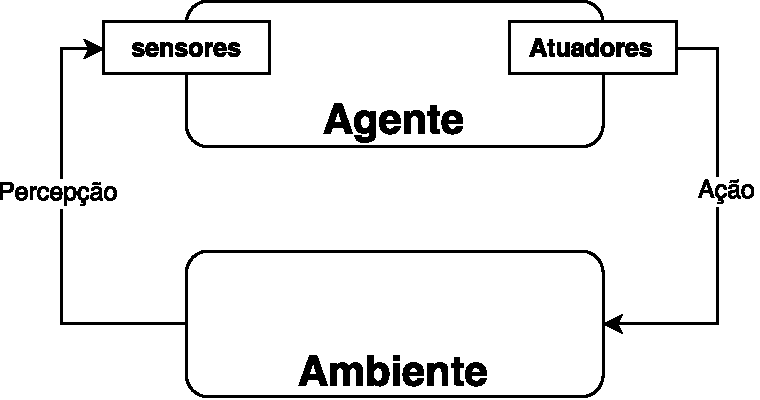
\includegraphics[width=0.4\textwidth]{fig/agente.pdf}
	\caption{Representação de um agente}
	\label{fig:agente}
\end{figure} 

Ao contrario dos objetos, os agentes são autônomos, podem aprender a lidar com as situações, e são ativos. Para que o agente consiga cumprir estes aspectos é preciso que ele seja capaz de realizar uma ação de forma autônoma e flexível, para que isso acontece, um agente precisa de três atributos\cite{agent1999}: 

\begin{itemize}
	\item Reatividade - Para que os agentes sejam capazes de perceber o ambiente e suas mudanças a fim de levar o ambiente em consideração para a tomada de decisão das ações;
	\item Pró-atividade - Para que os agentes consigam ter a iniciativa em tomar as suas ações;
	\item Habilidade social - Para que os agentes sejam capazes de interagir com outros agentes(humanos ou não).
\end{itemize}

Os dois primeiros atributos são mais intuitivos pelo que já foi explicado antes, o ultimo vem do fato de que um agente nem sempre vai estar sozinho no ambiente. Quando isso acontece temos o que é chamado de Sistemas multi agentes, que é um sistema onde temos mais de um agente e eles interagem um com os outros. Os agentes podem ter objetivos em comum ou não, mas o mais importante é que eles terão que, dependendo da situação, cooperar ou negociar entre si \cite{intelligence2003modern}.    
